\subsection{Specyfikacja wymagań na produkt programowy}

\begin{figure}[!htb]
    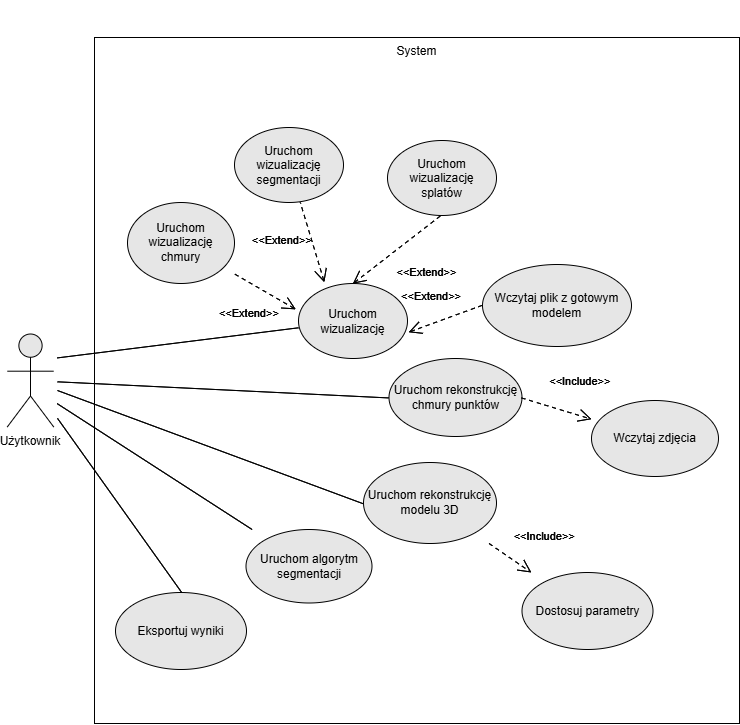
\includegraphics[width=1.0\linewidth]{img/diagramy/zpi use case.png}
    \caption{Diagram przypadków użycia}\label{fig:use_case_diagram}
  \end{figure}

\subsection{Architektura}

\begin{figure}[!htb]
    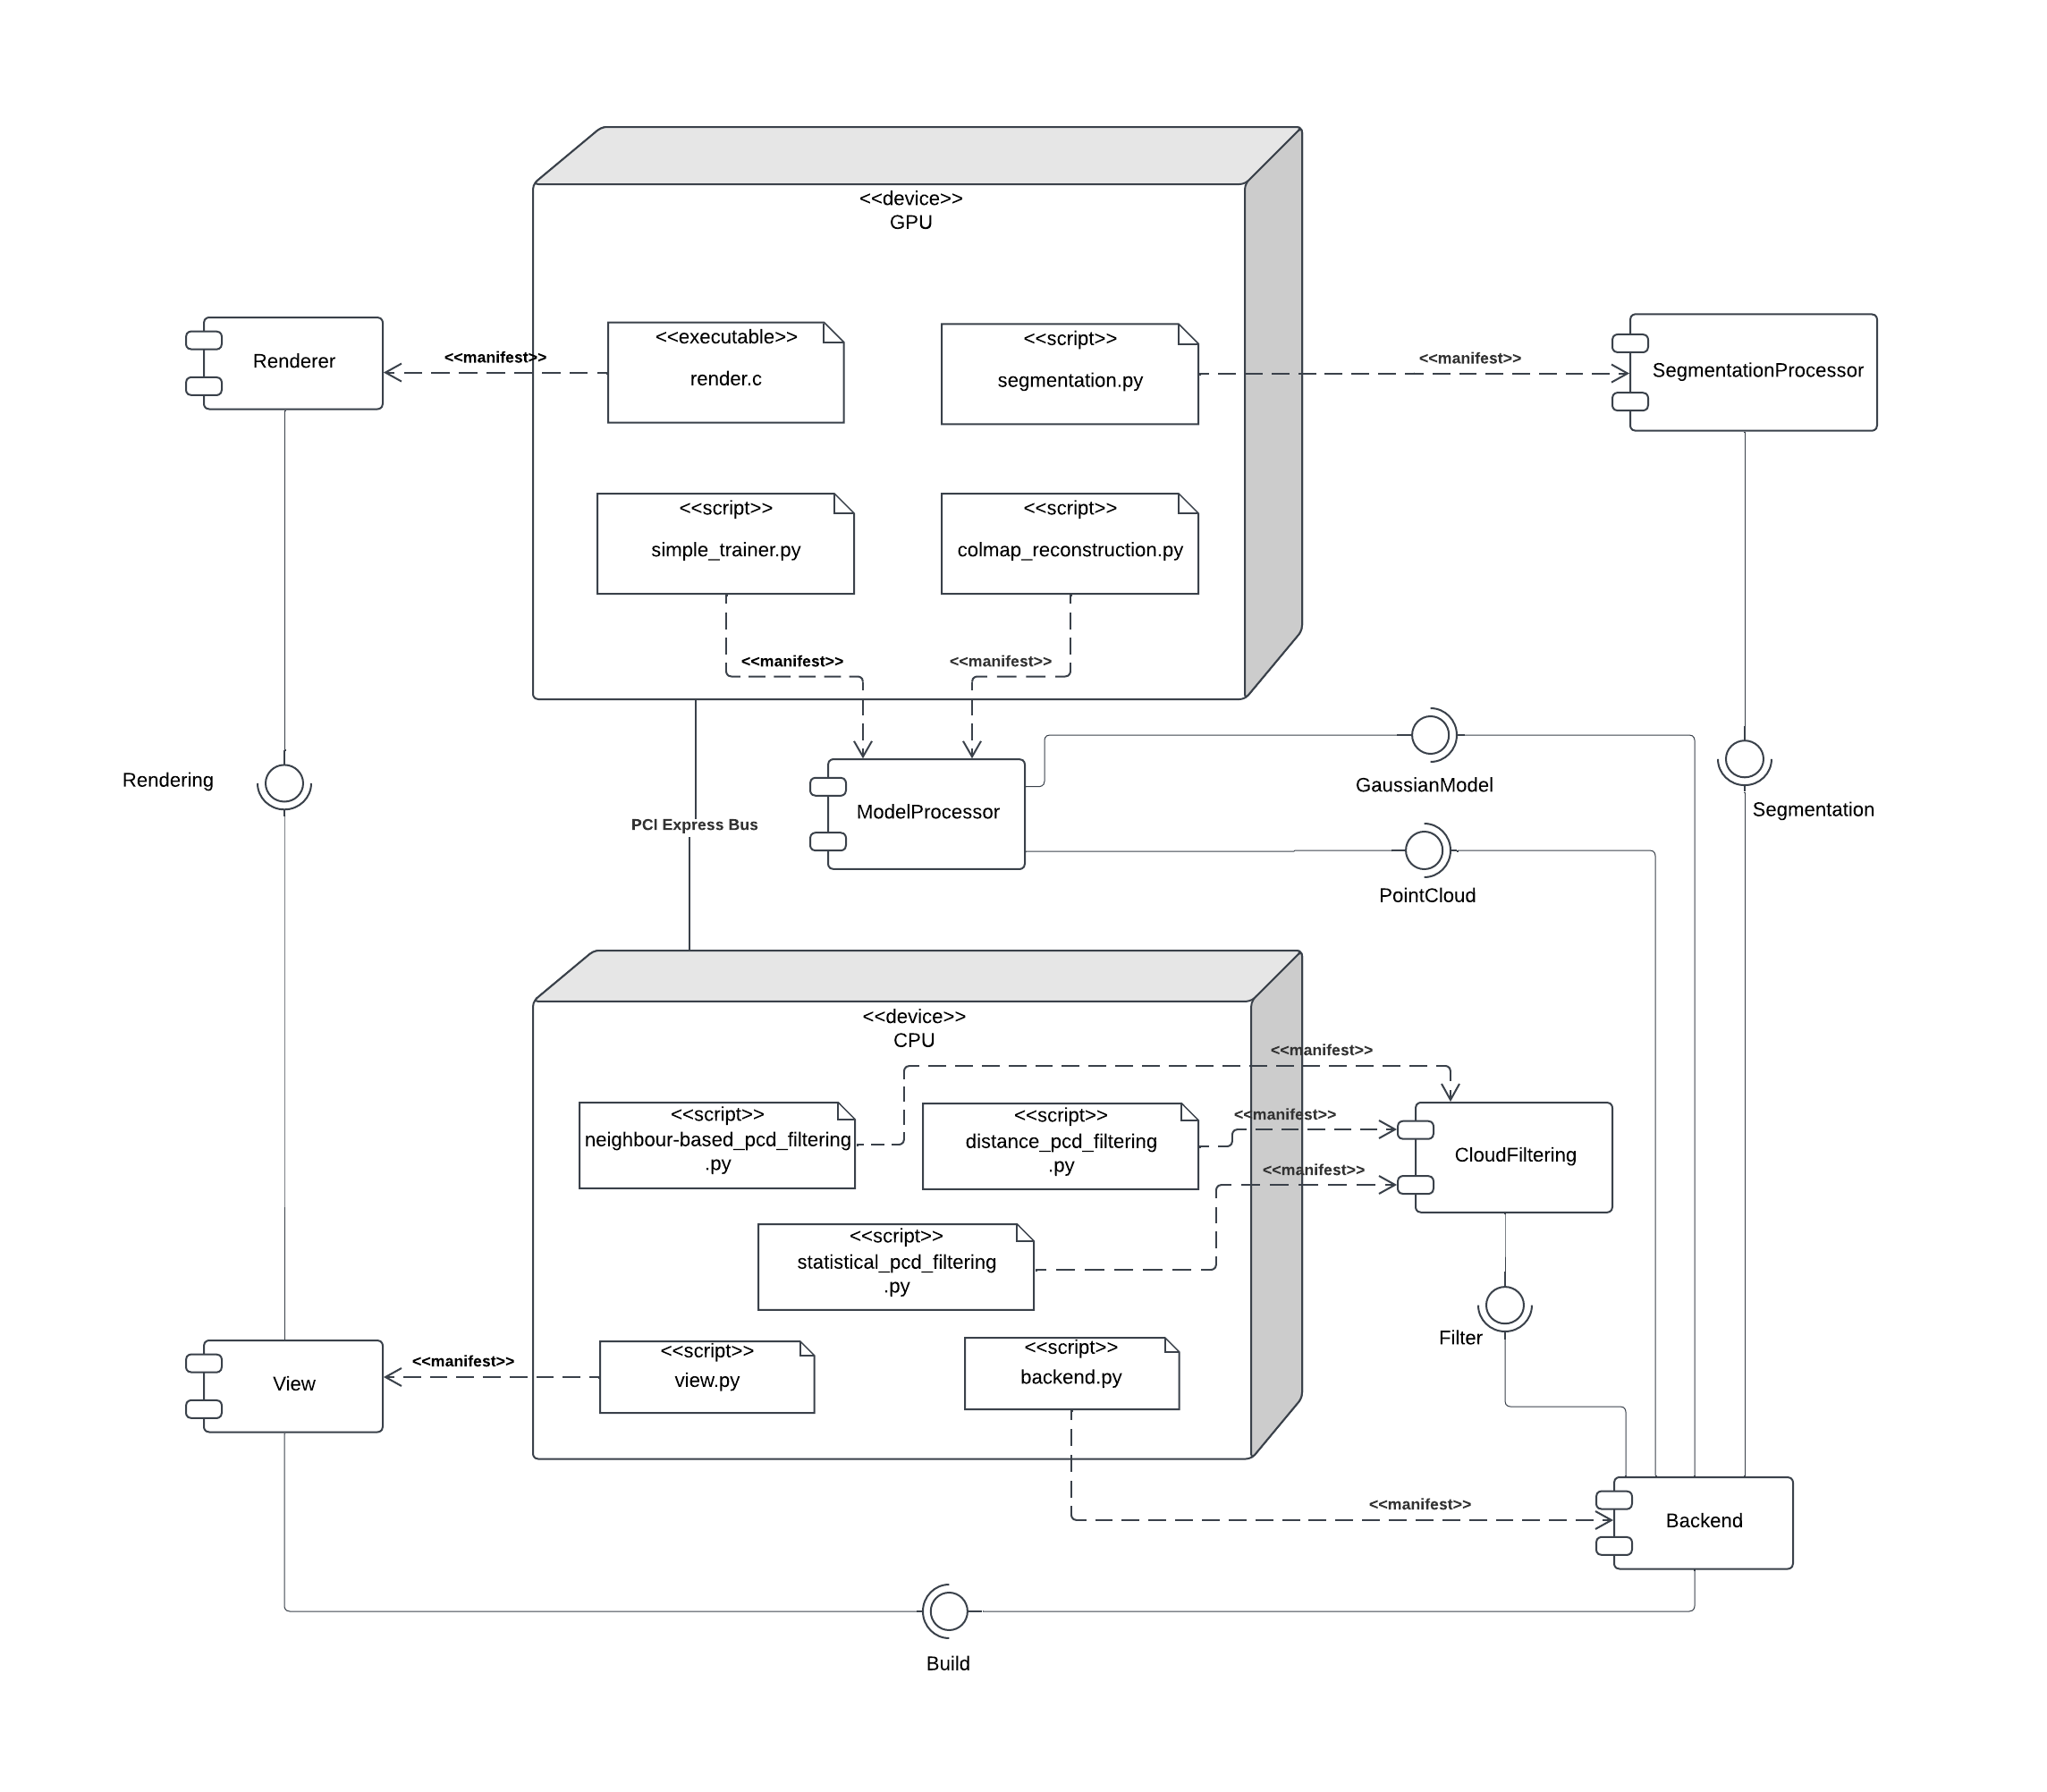
\includegraphics[width=1.0\linewidth]{img/diagramy/diagram_wdrozenia_komponentow_3.png}
    \caption{Diagram wdrożenia komponentów}\label{fig:components_diagram}
\end{figure}


\subsection{Implementacja}

\subsection{Technologie}

W projekcie wykorzystano następujące technologie

\begin{itemize}
    \item \textbf{C/C++}: OpenCL, OpenGL
    \item \textbf{Python}: Pytorch, pycolmap, open3d, pyvista, PyQt (numpy, matplotlib), pytest
    \item CloudCompare, Meshlab
    \item \textbf{GPU}
    \item Jira, Confluence, Github, Discord
\end{itemize}

\begin{figure}[!ht]
    \centering
    
\includegraphics[width=0.9\linewidth]{img/sota/technologie.png}
  \end{figure}

\subsubsection{Struktura plikowa projektu}

% millon opcji https://tex.stackexchange.com/questions/5073/making-a-simple-directory-tree
\begin{forest}
  for tree={
    grow'=0,
    child anchor=west,
    parent anchor=south,
    anchor=west,
    calign=first,
    edge path={
      \noexpand\path [draw, \forestoption{edge}] (!u.south west) ++(3pt,0) -- +(-3pt,0) |- (.child anchor)\forestoption{edge label};
    },
    before typesetting nodes={
      if n=1
        {insert before={[,phantom]}}
        {}
    },
    fit=band,
    before computing xy={l=15pt},
  }
[project
  [data
    [city\_model
      [images]
      [sparse
          [images.bin]
          [cameras.bin]
          [points.bin]
          [sparse.ply]
      ]
      [filtered\_model.ply]
      [model.pt]
      [model.ply]
      [model\_seg.ply]
    ]
    [pointnet-ckpt.pt]
  ]
  [scripts]
  [src
    [frontend]
    [backend]
    [urb3d
      [datasets]
      [pipeline]
      [segmentation]
      [rendering]
      [geometry]
      [models]
      [splats]
    ]
  ]
  [test]
]
\end{forest}